%%%%%%%%%%%%% Appendices %%%%%%%%%%%%%


\chapter{Appendix}
All the relevant files and progress data is available in \href{https://github.com/dakshinatharindu/Hot-Plate.git}{this} Github repository.
\section{The PCB}
Schematics, PCB and table of content.
Used Altium Designer to design these models
%\includegraphics[]{Appendix/Alarm_Clock.pdf}


  \begin{figure}
  \noindent\makebox[\textwidth]{
  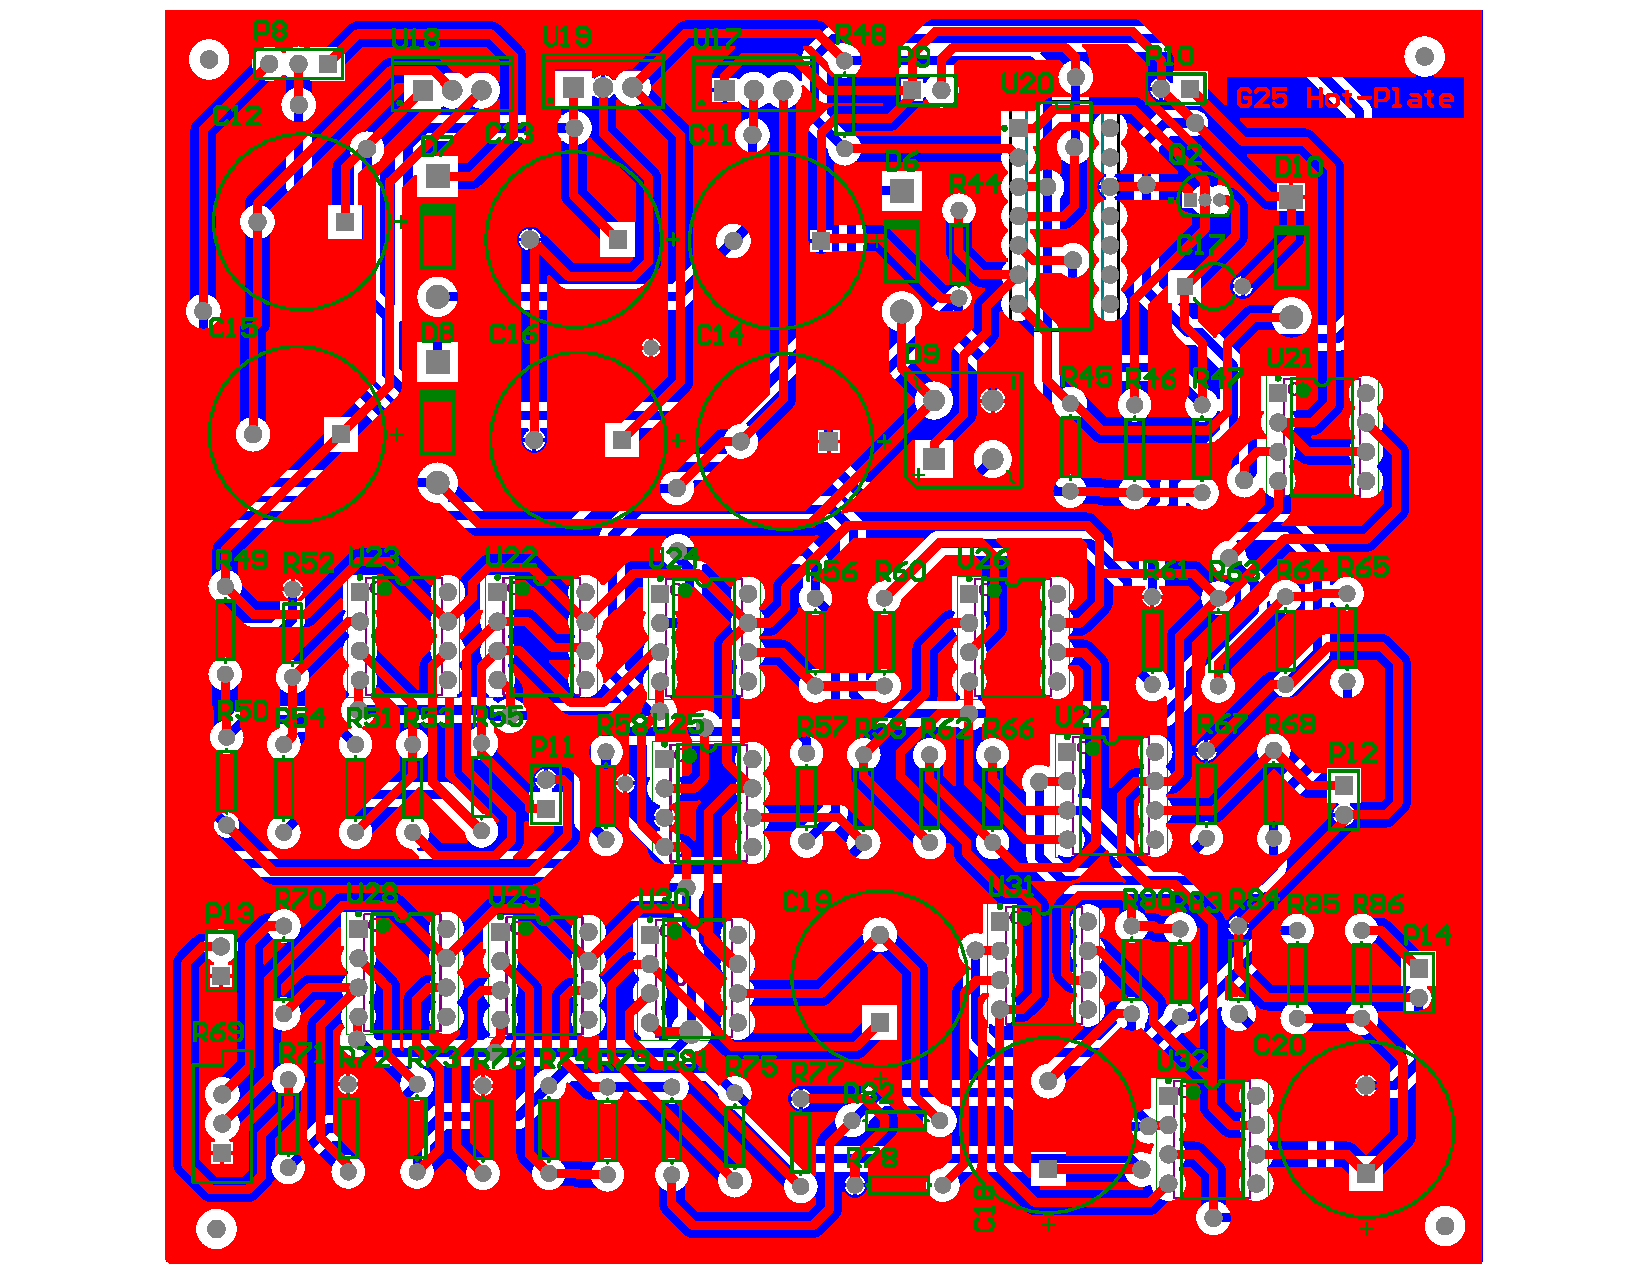
\includegraphics[width=1\textwidth,page=1]{PCB fabricated/PCB2.pdf}}
  \caption{PCB Design - Top Layer}
\end{figure}

  \begin{figure}
  \noindent\makebox[\textwidth]{
  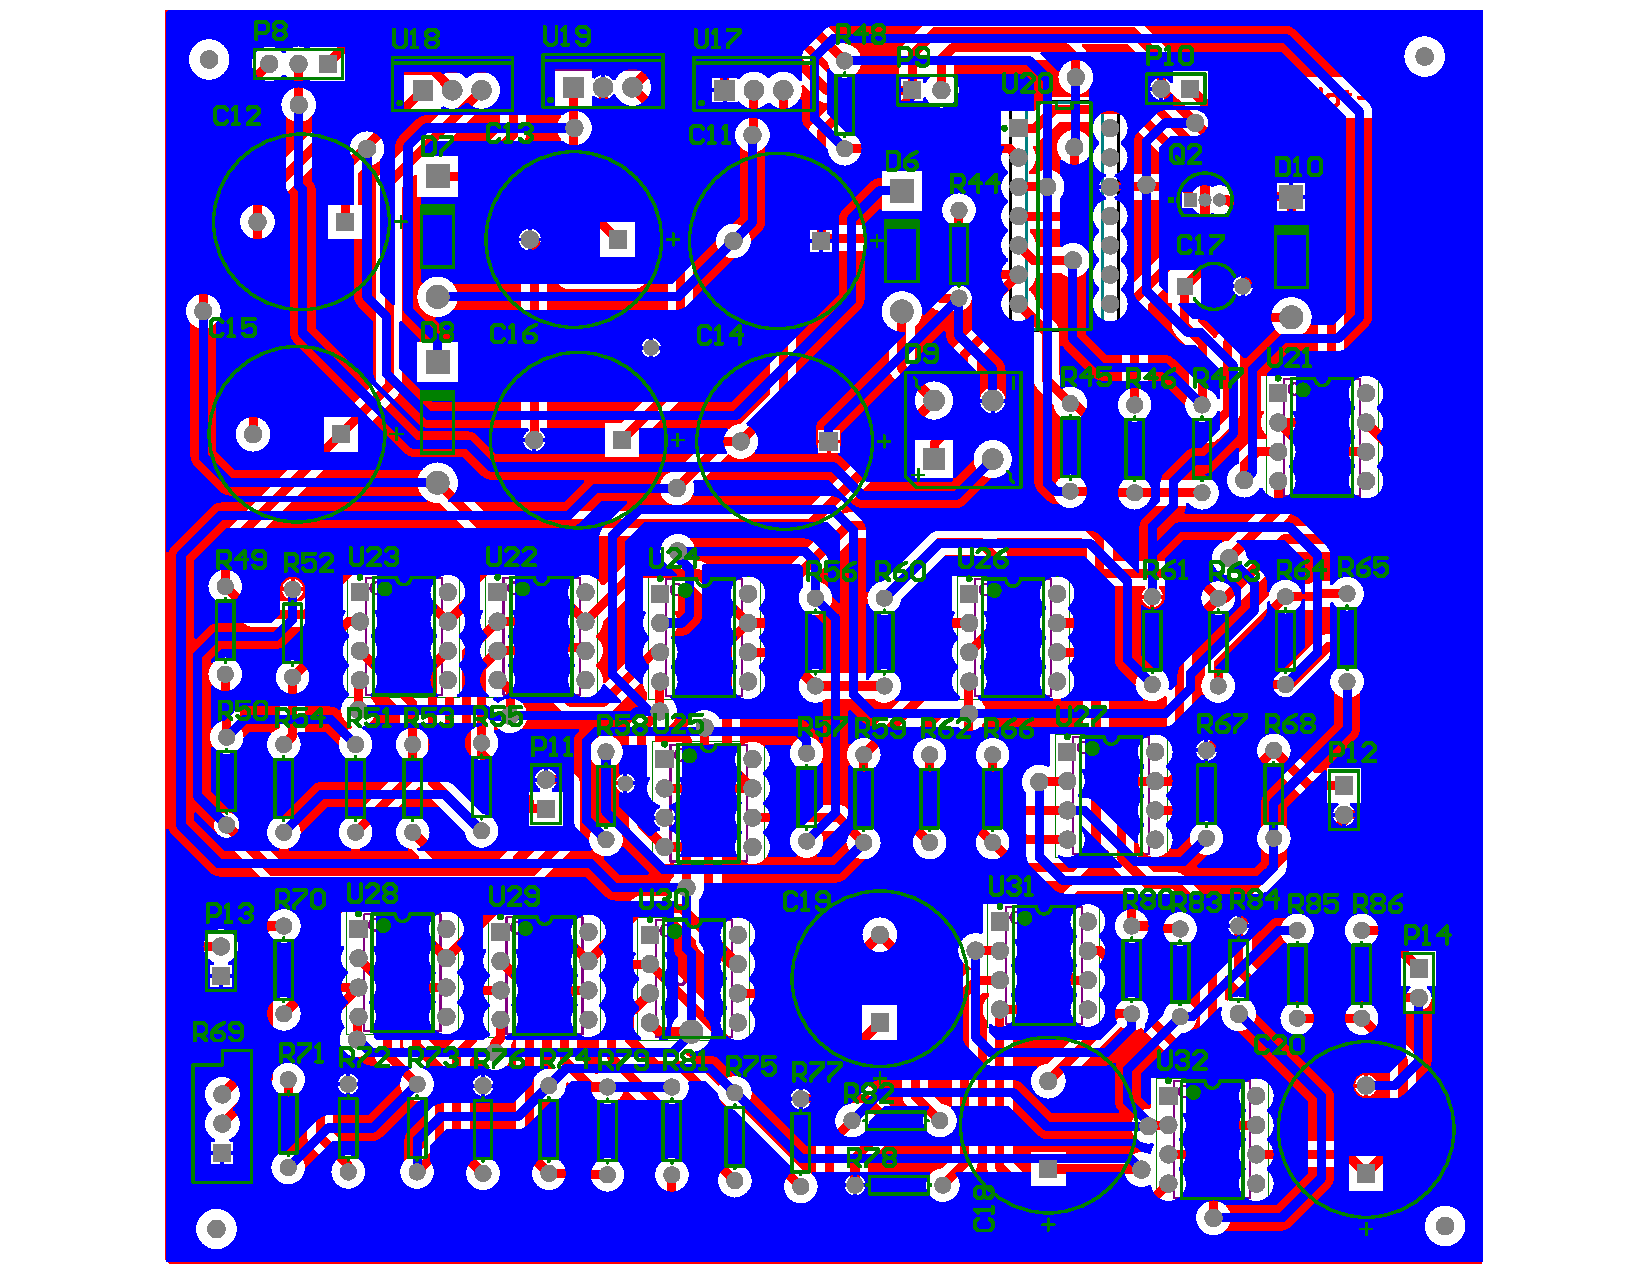
\includegraphics[width=1\textwidth,page=1]{PCB fabricated/PCB1.pdf}}
  \caption{PCB Design - Bottom Layer}
\end{figure}

  \begin{figure}
  \noindent\makebox[\textwidth]{
  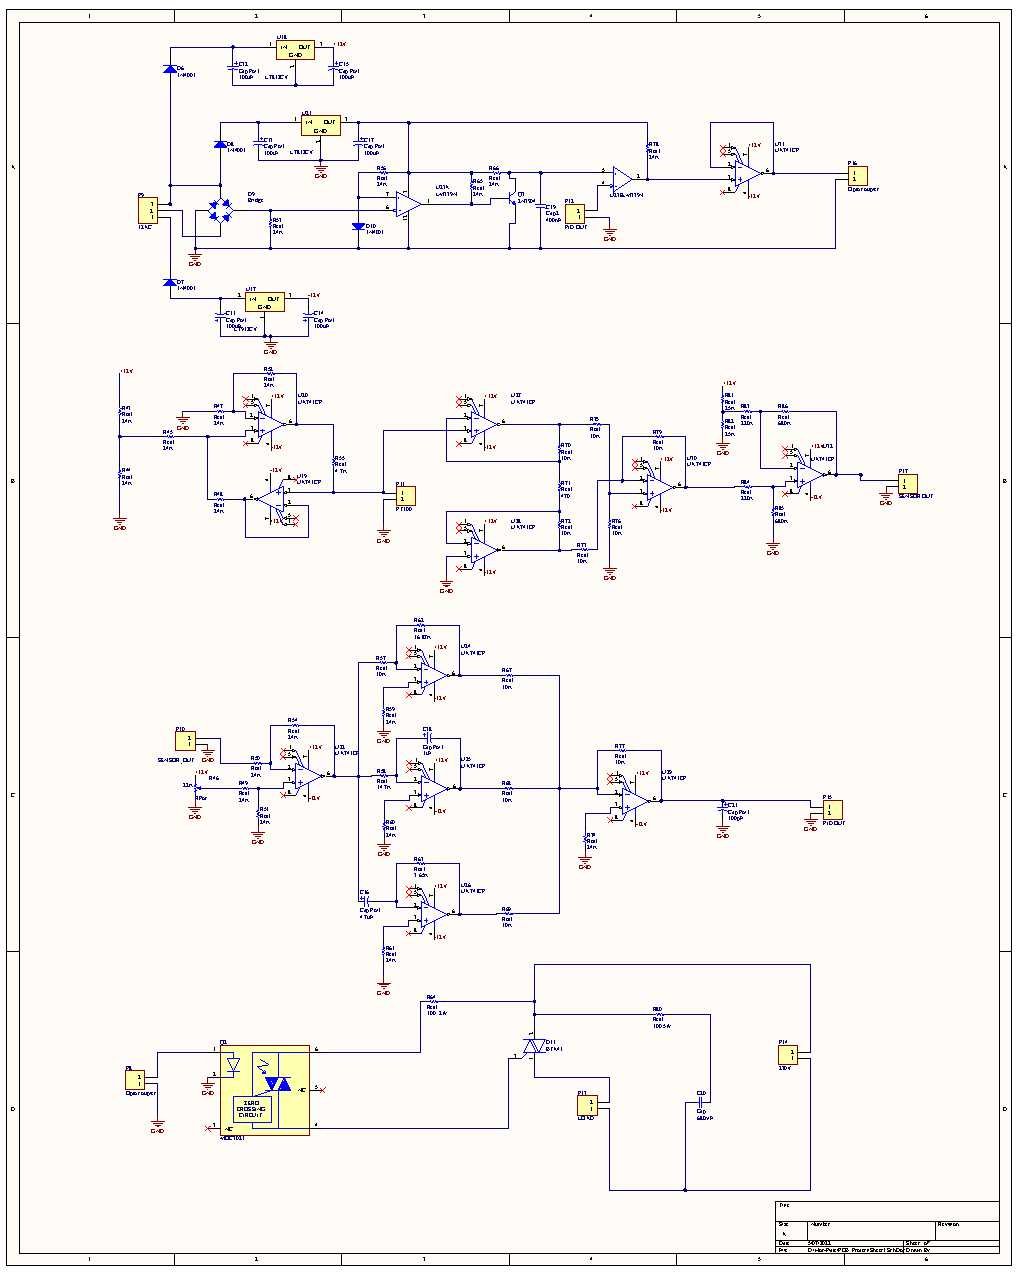
\includegraphics[width=1\textwidth,page=1]{PCB fabricated/schematic.pdf}}
  \caption{Schematics Design}
\end{figure}
\newpage
\section{Proteus schematics}

  \begin{figure}[h]
  \noindent\makebox[\textwidth]{
  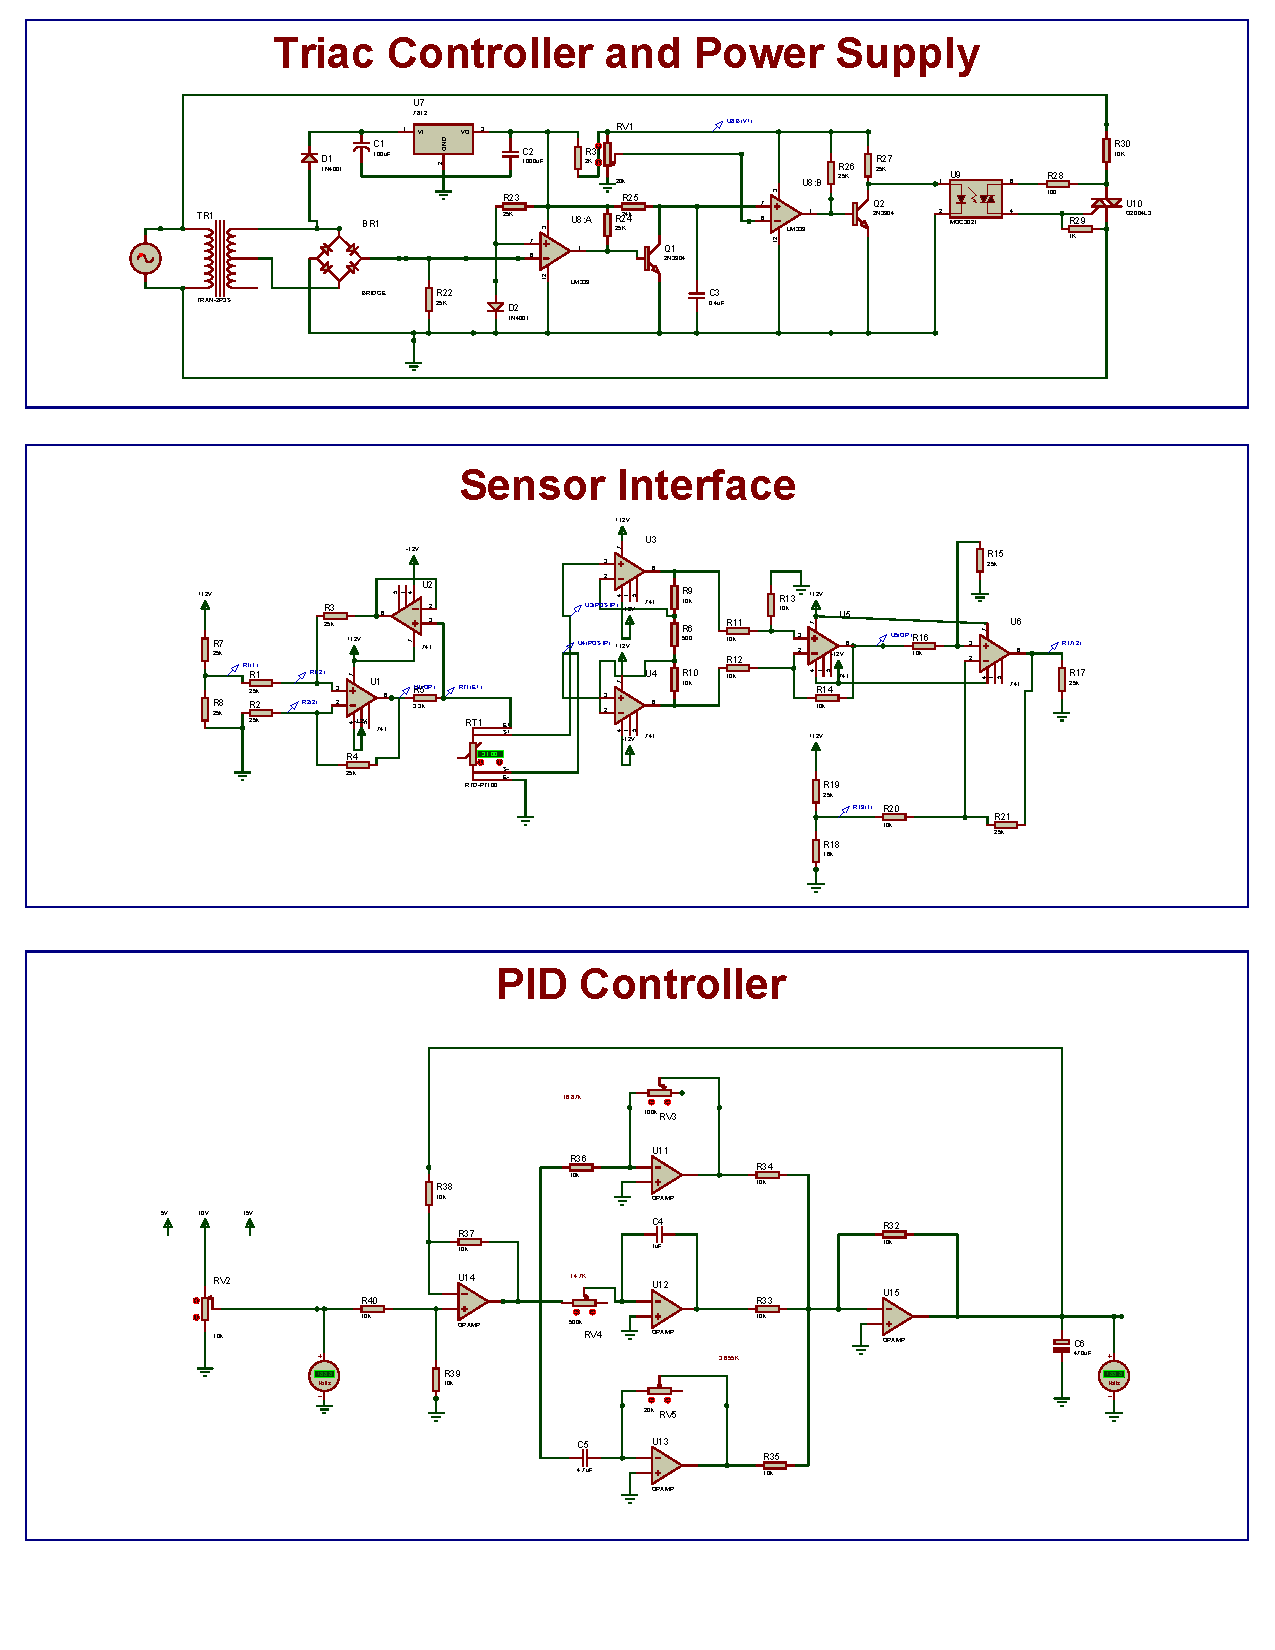
\includegraphics[width=0.85\textwidth,page=1]{PCB fabricated/proteus.pdf}}
  \caption{Proteus Simulation}
\end{figure}
\newpage

\section{Enclosure}

\begin{figure*}[h]
        \centering
        \begin{subfigure}{0.475\textwidth}
            \centering
            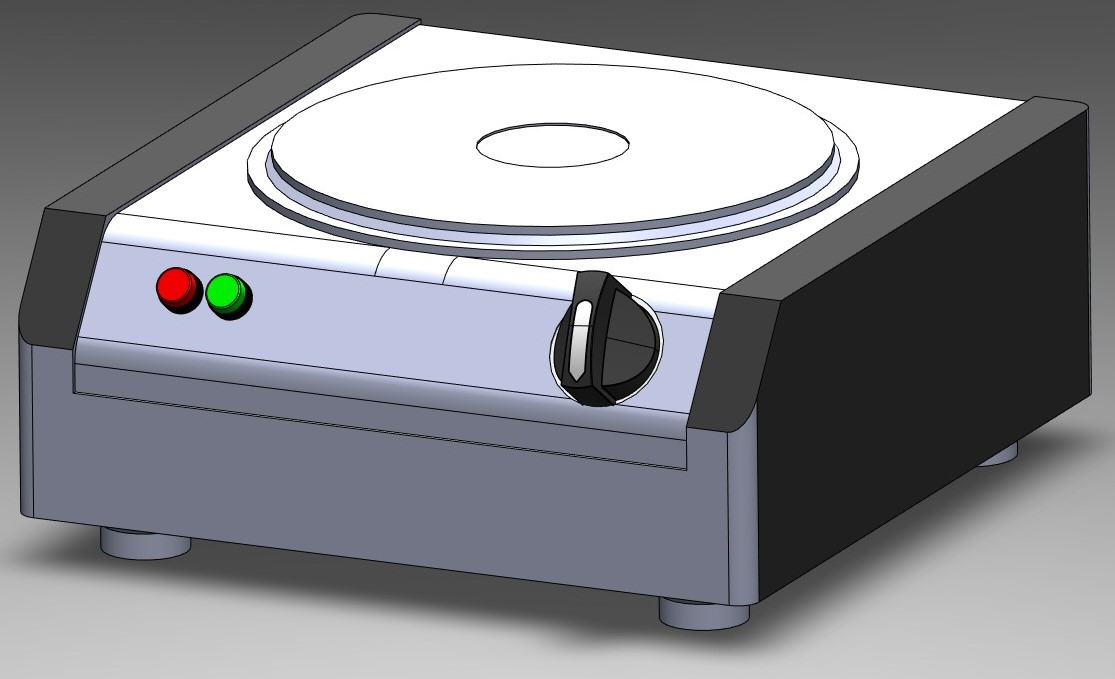
\includegraphics[width=\textwidth]{Enclosure/01969125-4170-495c-98ca-1aa0abf50a48 - Copy.JPG}
        \end{subfigure}
        \hfill
        \begin{subfigure}{0.475\textwidth}  
            \centering 
            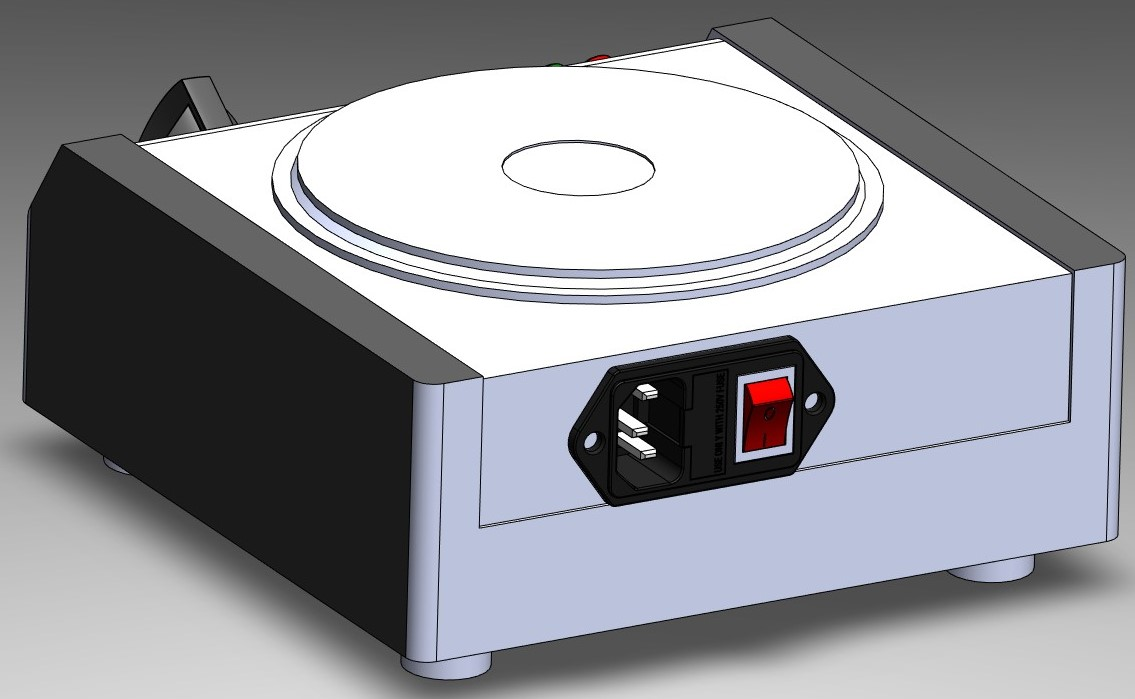
\includegraphics[width=\textwidth]{Enclosure/16bace9b-620b-4e5d-a89f-7e68709594fe.JPG}
            
        \end{subfigure}
        \vskip\baselineskip
        \begin{subfigure}{0.475\textwidth}   
            \centering 
            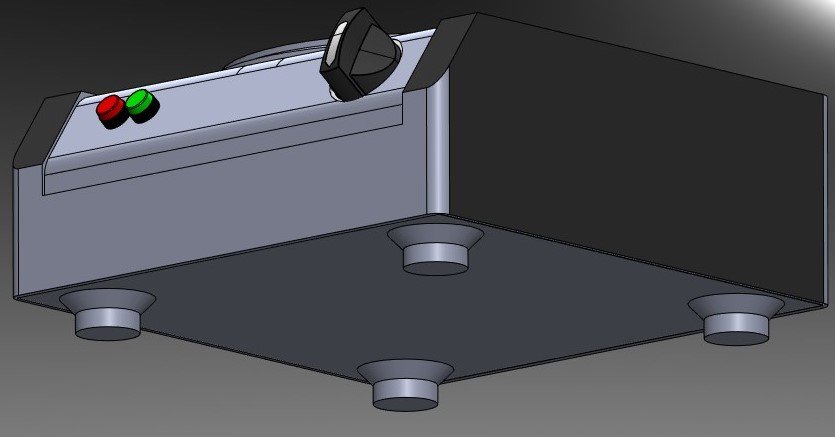
\includegraphics[width=\textwidth]{Enclosure/9b6e8738-6aa5-4382-9c02-1e854646a67c.JPG}
            
        \end{subfigure}
        \hfill
        \begin{subfigure}{0.475\textwidth}   
            \centering 
            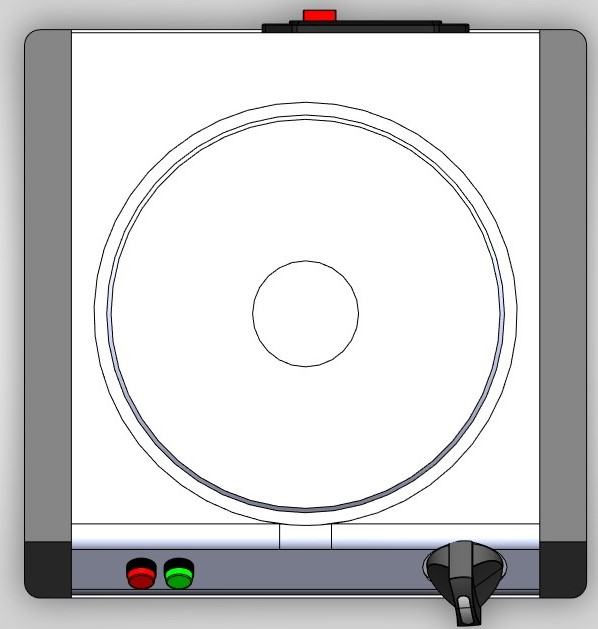
\includegraphics[width=\textwidth]{Enclosure/e37a053d-cc5b-4a5f-88a6-e2852106d6c8.JPG}
            
        \end{subfigure}
        \caption[ The average and standard deviation of critical parameters ]
        {\small Solidworks Enclosure} 
        \label{fig:mean and std of nets}
    \end{figure*}
